\chapter[Fundamentação Teórica]{Fundamentação Teórica}
\label{cp:fundamentacao}

\section{Gerenciamento de Projetos}
\label{sec:gerenciamento_de_projetos}

\subsection{Modelo Tradicional - PMBOK}
\label{sec:modelo_tradicional}

Uma metodologia de gerenciamento de projetos no modelo tradicional, de acordo com \citeonline{kerzner} é o alcance da excelência no controle dos projetos e que se torna impossível sem um processo repetitivo que possa ser utilizado em cada projeto.

No modelo tradicional, um dos modelos utilizados é o definido no \citeonline{pmbok}. \citeonline{gerenciamento_de_projetos_pmbok} define gerenciamento de projetos como uma interação de ações, em que a falta de alguma ação, pode afetar também outras áreas. Essas interações podem levar a mudanças no projeto, dependendo do seu tamanho, e mudanças quase sempre afetam o prazo de entrega do projeto, e elevam os custos. O PMBOK (\textit{Project Management Body of Knowledge}) possui cinco grupos de processos, como pode ser na Figura \ref{img:fases_pmbok}:

\begin{figure}[H]
	\centering
	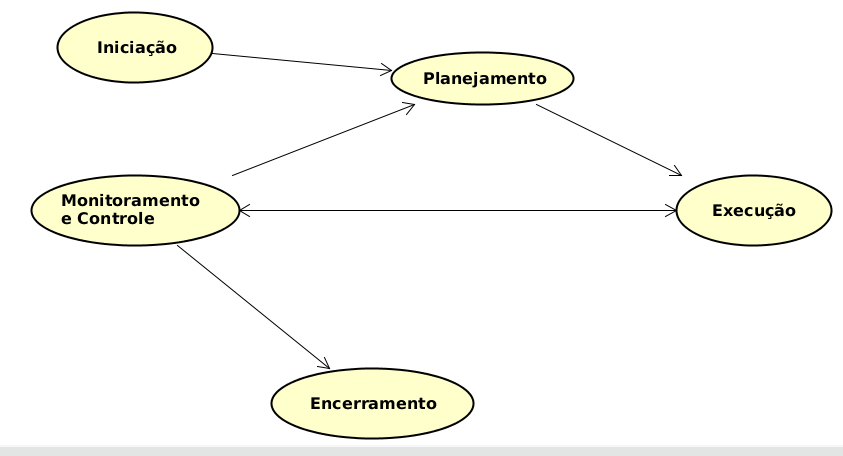
\includegraphics[width=0.8\textwidth]{figuras/fases_pmbok.png}
	\caption{Grupos de processos do Gerenciamento de Projetos, Fonte: Própria.}
	\label{img:fases_pmbok}
\end{figure}

A definição desses grupos de processos podem ser vistos a seguir:

\begin{itemize}
	\item \textbf{Processos de Iniciação} – reconhecer que um projeto ou fase deve começar e se comprometer para executá-lo(a);
	\item \textbf{Processos de Planejamento} – planejar um esquema de trabalho que seja viável para atingir os objetivos do projeto;
	\item \textbf{Processos de Execução} – Coordenar pessoas e recursos para implementar o plano;
	\item \textbf{Processos de Monitoramento e Controle} – Averiguar que os objetivos do projeto estão sendo seguidos, monitorados e avalia-los segundo seu progresso, realizando ações corretivas e replanejando sempre que necessário; 
	\item \textbf{Processos de Encerramento} – formalizar a aceitação do projeto ou
	fase e encerra-lo(a) de uma forma organizada.
\end{itemize}

Esses processos são ligados pelos resultados que são desenvolvidos neles, sendo que a saída de um processo é a entrada de outro processo. O desenvolvimento do plano de gerenciamento do projeto é uma atividade iterativa ao longo do ciclo de vida do projeto, sempre pronto para melhoria contínua e permitindo à equipes do projeto definir e trabalhar com maior nível de detalhes. De acordo com o \citeonline{pmbok} podem ser sobrepostas, ou seja, o início de uma fase é ao término de uma outra, isso leva a algumas atividades ocorrerem de forma paralela. A maneira como este tipo de projeto é definido, aumenta os riscos, retrabalhos, e exige recursos adicionais para permitir que as atividades ocorram em paralelo, como mostrado na Figura \ref{img:fases_sobrepostas}.

\begin{figure}[H]
	\centering
	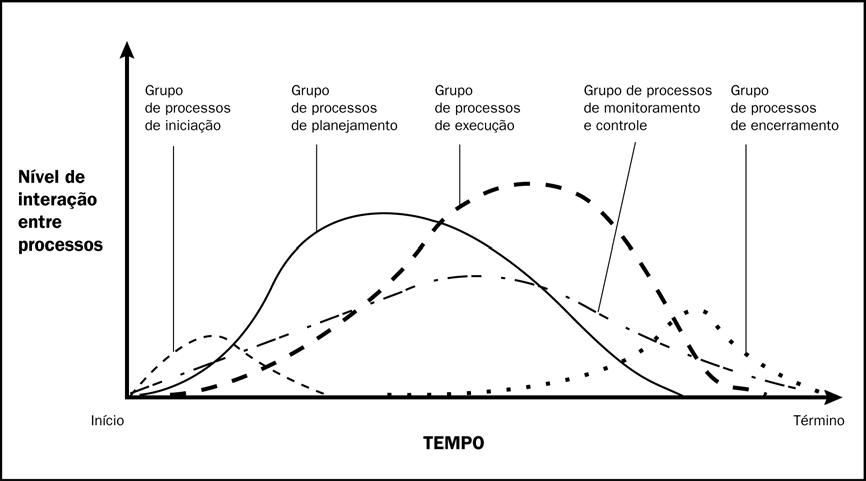
\includegraphics[width=0.8\textwidth]{figuras/fases_pmbok_sobrepostas.jpg}
	\caption{Superposição dos Grupos de Processo. Fonte: \citeonline{fases_sobrepostas_pmbok}.}
	\label{img:fases_sobrepostas}
\end{figure}

\subsubsection{Áreas de Conhecimento PMBOK}

O PMBOK, na versão 5, possui nove áreas de conhecimentos, sendo elas:

\begin{itemize}
	\item \textbf{Gerência da Integração do Projeto} - descreve os processos necessários para que os diversos elementos do projeto sejam adequadamente coordenados. Responsável pelo desenvolvimento do plano do projeto, execução do plano do projeto e controle das mudanças;
	\item \textbf{Gerência do Escopo do Projeto} - descreve os processos necessários para que o projeto atenda ao que foi definido no inicio do projeto, e nada além disso. Contempla a fase de iniciação, planejamento, detalhamento, verificação e controle de mudanças do escopo;
	\item \textbf{Gerência do Tempo do Projeto} - descreve os processos necessários para que o projeto seja concluido dentro do prazo previamente estabelecido. Definição, sequenciamento e estimação das atividades, além do cronograma fazem parte dessa área;
	\item \textbf{Gerência do Custo do Projeto} - descreve os processos necessários para assegurar que o projeto seja completado dentro do orçamento previsto. Supervisiona o planejamento dos recursos, estimativa, orçamento e controle dos custos;
	\item \textbf{Gerência da Qualidade do Projeto} - descreve os processos necessários para assegurar que as necessidades que originaram o desenvolvimento do projeto serão
	satisfeitas. Abrange o planejamento, garantia e controle da qualidade;
	\item \textbf{Gerência dos Recursos Humanos do Projeto} - descreve os processos necessários para proporcionar a melhor utilização das pessoas envolvidas no projeto. Responsável pelo planejamento organizacional, montagem e desenvolvimento da equipe;
	\item \textbf{Gerência das Comunicações do Projeto} - descreve os processos necessários para assegurar que a geração, captura, distribuição, armazenamento e pronta apresentação das informações do projeto sejam feitas de forma adequada e no tempo certo. Ela é composta pelo planejamento das comunicações, distribuição das
	informações, relato de desempenho e encerramento administrativo.
	\item \textbf{Gerência dos Riscos do Projeto} - descreve os processos que dizem respeito à identificação, análise e resposta a riscos do projeto. É composta pela identificação, quantificação, desenvolvimento das respostas e controle das respostas aos riscos.
	\item \textbf{Gerência das Aquisições do Projeto} - descreve os processos necessários para a aquisição de mercadorias e serviços fora da organização que desenvolve o projeto. É responsável pelo planejamento, preparação das aquisições, obtenção de propostas, seleção de fornecedores, administração dos contratos e encerramento do contrato.
\end{itemize}

Este modelo de gerenciamento de projeto é mais voltado em empresas já consolidadas, de ramo mais formal, que possui mais burocracia em seus projetos e por tanto maior rigor de documentação e de liderança dos gerentes. Essa hierarquia pode ser vista na Figura \ref{img:gerencia_de_projetos_tradicional}.

\begin{figure}[H]
	\centering
	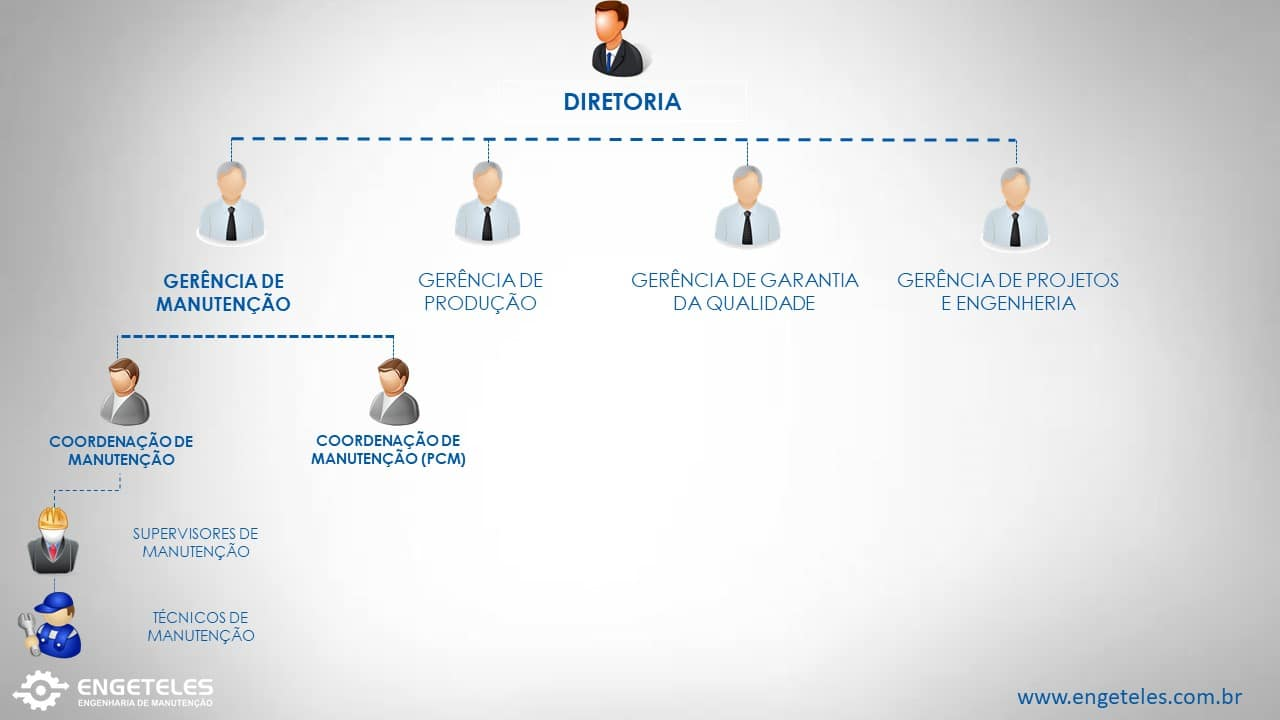
\includegraphics[width=0.8\textwidth]{figuras/gerencia_de_projeto.jpg}
	\caption{Hierarquia em projetos tradicionais. Fonte: \citeonline{gerentes_tradicionais}.}
	\label{img:gerencia_de_projetos_tradicional}
\end{figure}

\subsubsection{Casos de Uso}
\label{sec:casos_de_uso}

Os casos de uso é uma das principais características presentes na linguagem de modelagem UML (\textit{Unified Modeling Language}), ou linguagem modelada unificada. \citeonline{sommerville} define os objetivos dos casos de uso como identificar os atores envolvidos e suas interações com o projeto. Os casos de uso é um diagrama de auto nível, ou seja, não possui uma linguagem técnica e o usuário final consegue entender sem dificuldades.

Na Figura \ref{img:exemplo_caso_de_uso} é possível visualizar um exemplo de caso de uso:

\begin{figure}[H]
	\centering
	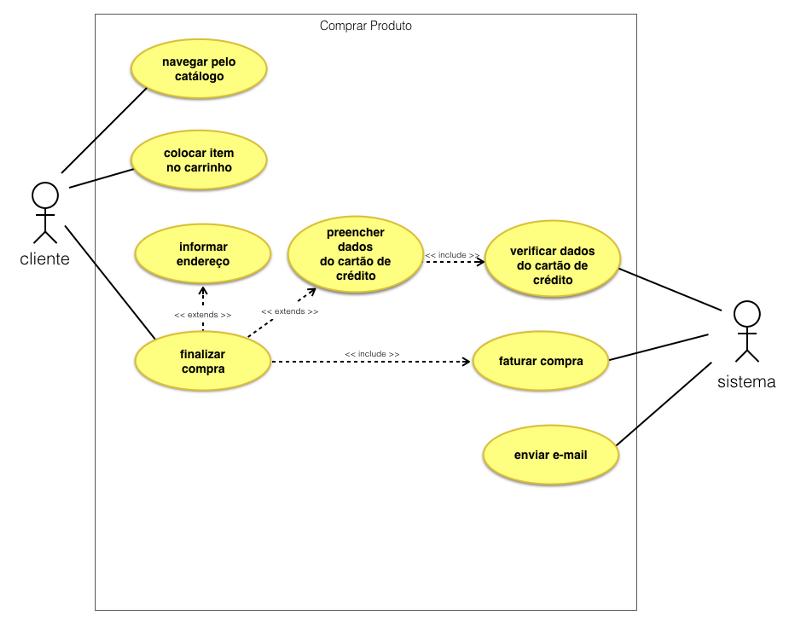
\includegraphics[width=0.7\textwidth]{figuras/caso_de_uso_exemplo.png}
	\caption{Exemplo de Caso de Uso. Fonte: \citeonline{casos_de_uso}.}
	\label{img:exemplo_caso_de_uso}
\end{figure}

\subsection{Modelo Ágil}
\label{sec:modelo_agil}

Em contraposição ao modelo tradicional, surge o manifesto ágil como uma reação contra o processo burocrático presente no PMBOK, que possuem por característica atividades sequências em modelo iterativo e cascata. Segundo a \citeonline{chaos} apenas 16,2\% dos projetos entregues por companhias americanas foram entregues respeitando prazos, custos previamente acordados e objetivos determinados. Segundo a própria \citeonline{chaos}, as principais causas destes problemas estavam relacionadas com o modelo sequencial tradicional.

No modelo ágil, segundo \citeonline{soares}, 
as mudanças são bem vindas, desde que ajude a entregar um projeto melhor. Cabe a equipe de gerência agir de maneira rápida, sabendo receber, avaliar e responder as mudanças  como elas devem ser atendidas e repassar suas consequências aos desenvolvedores e clientes. As principais características da metodologia ágil são:

\begin{itemize}
	\item Desenvolvimento iterativo e incremental;
	\item Comunicação;
	\item Documentação reduzida; 
\end{itemize}

Em 2001, membros da comunidade de \textit{software} se reuniram e criaram o \citeonline{agile_manifest}. O objetivo deste manifesto é utilizar as melhores práticas observadas em projetos anteriores que obtiveram sucessos.

Os principais conceitos do manifesto ágil são:

\begin{itemize}
	\item Indivíduos e interações ao invés de processos e ferramentas;
	\item \textit{software} executável ao invés de documentação;
	\item colaboração do cliente ao invés de negociação de contratos;
	\item resposta rápida a mudanças ao invés de seguir planos pré-estabelecidos.
\end{itemize}

No modelo ágil os requisitos dos clientes podem ser mudados a qualquer momento, e o time de gerência e desenvolvimento devem estar preparados para conversar com o cliente a fim de resolver as alterações de requisitos da melhor maneira possível. Este tipo de pensamento no modelo tradicional é mais difícil de acontecer, pois neste modelo é possível notar que ao iniciar uma fase, essa mesma fase não é retornada mais tarde, ou seja, no modelo tradicional uma troca de requisitos pode levar ao reinicio do projeto, ou a um produto final que não atenda mais a necessidade do cliente.

Este modelo ágil é mais focado para empresas emergentes, que não são muito rigorosas em seus processos e aceita que mudanças nos requisitos ou na visão do produto são sempre bem vindas, desde que melhore o projeto final.

\subsubsection{Scrum}
\label{sec:scrum}

Uma das boas práticas adotadas ao modelo ágil é o \textit{Scrum}. O \textit{Scrum}, é um \textit{framework} que se refere ao jogo \textit{Rugby}, em que os jogadores para avançar, devem avançar no campo e planejar de forma conjunta. Essa ação de planejamento conjunto, aumenta o engajamento dos envolvidos no projeto. Um dos principais pontos de vista do \textit{Srum} é planejar um projeto com pequenos ciclos e aumentar as interações entre os participantes, mas com visão a longo prazo.

O ciclo de vida de um projeto \textit{Scrum} pode ser visto na figura \ref{img:ciclo_de_vida_scrum}:

\begin{figure}[H]
	\centering
	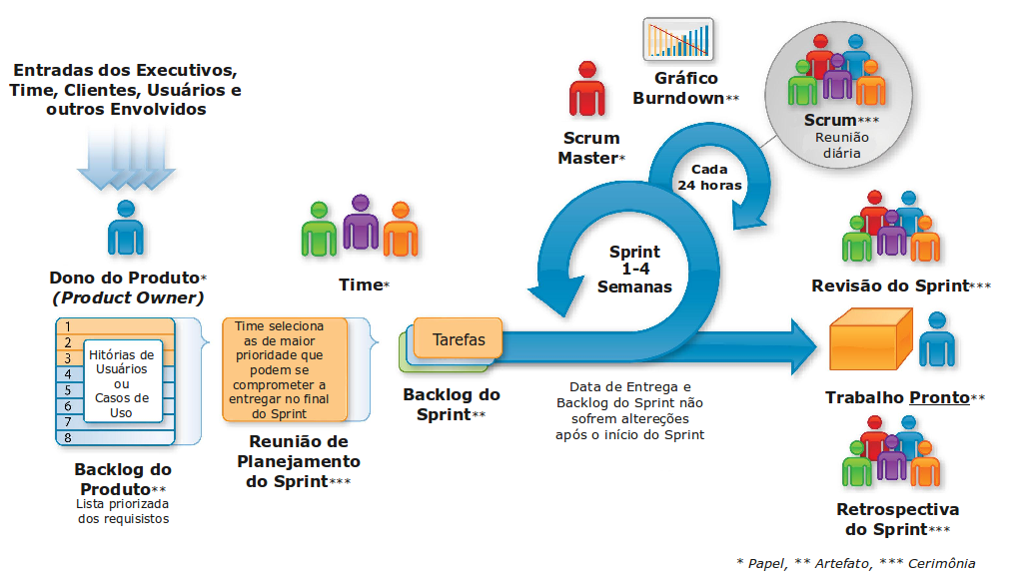
\includegraphics[width=0.8\textwidth]{figuras/ciclo_de_vida_scrum.png}
	\caption{Ciclo de Vida SCRUM. Fonte: \citeonline{scrum}.}
	\label{img:ciclo_de_vida_scrum}
\end{figure}

Como pode ser visto na figura \ref{img:ciclo_de_vida_scrum}, o \textit{Scrum} é um ciclo progressivo de várias iterações bem definidas, denominadas \textit{Sprints}. As \textit{Sprints} podem ter duração de uma a quatro semanas. Antes de cada \textit{Sprint}, deve ser realizada a reunião de planejamento da \textit{Sprint}, chamada de \textit{Sprint Planning Meeting}. A \textit{Sprint Planning Meeting} é uma reunião de planejemanto em que o \textit{Product Owner}
prioriza os itens do \textit{Product Backlog} e a equipe seleciona as atividades que serão implementadas ao longo da \textit{Sprint}. No \textit{Product Backlog} são registradas as funcionalidades que serão implementadas pedidas pelo \textit{Product Backlog}. 

Com o objetivo de saber o progresso de cada equipe dentro da \textit{Sprint}, ocorrem as reuniões diárias, denominadas \textit{Daily Meetings}, que tem duração de no máximo 15 minutos e ocorrem com todos os participantes em pé, respondendo perguntas como: "O que você fez ontem?", "O que você fez hoje?" e "O que você vai fazer amanhã?". 

Ao final de uma \textit{Sprint} é feita uma análise gráfico do progresso do projeto atráves do \textit{Sprint Backlog} durante a \textit{Sprint Review}. Após a \textit{Sprint Review} ocorre a \textit{Sprint Retrospective} que é a análise de experiências que ocorreram durante a \textit{Sprint} sejam boas ou não a fim de melhora-las.

Segundo \citeonline{fowler}, as equipes devem possuir um quadro para registro das atividades, denominado \textit{Kanban}. O \textit{Kanban} possui o objetivo de auxiliar as equipes em relação ao progresso da \textit{Sprint}, esse quadro pode ser dividido em 4 fases:

\begin{itemize}
	\item Para fazer;
	\item Em andamento (com o nome do responsável pela atividade);
	\item Em revisão;
	\item Feito.
\end{itemize}

\begin{figure}[H]
	\centering
	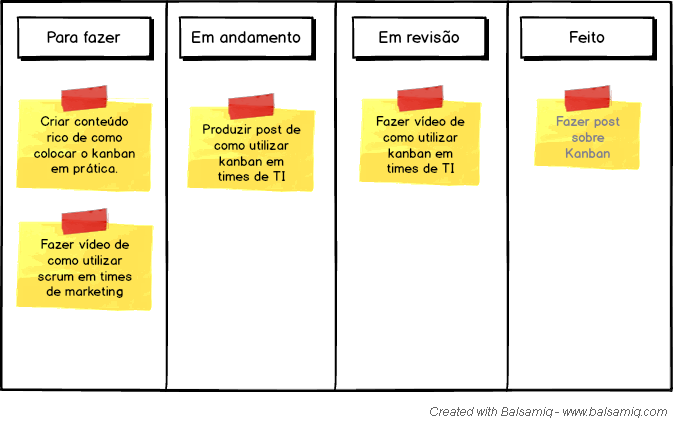
\includegraphics[width=1.0\textwidth]{figuras/kanban.png}
	\caption{Quadro Kanban. Fonte: \citeonline{kanban}.}
	\label{img:kanban}
\end{figure}

O \textit{Scrum} possui seus papéis bem definidos, podendo ser alterados ao longo do desenvolvimento do projeto. Esses papéis podem ser vistos na figura \ref{img:papeis_scrum}.

\begin{figure}[H]
	\centering
	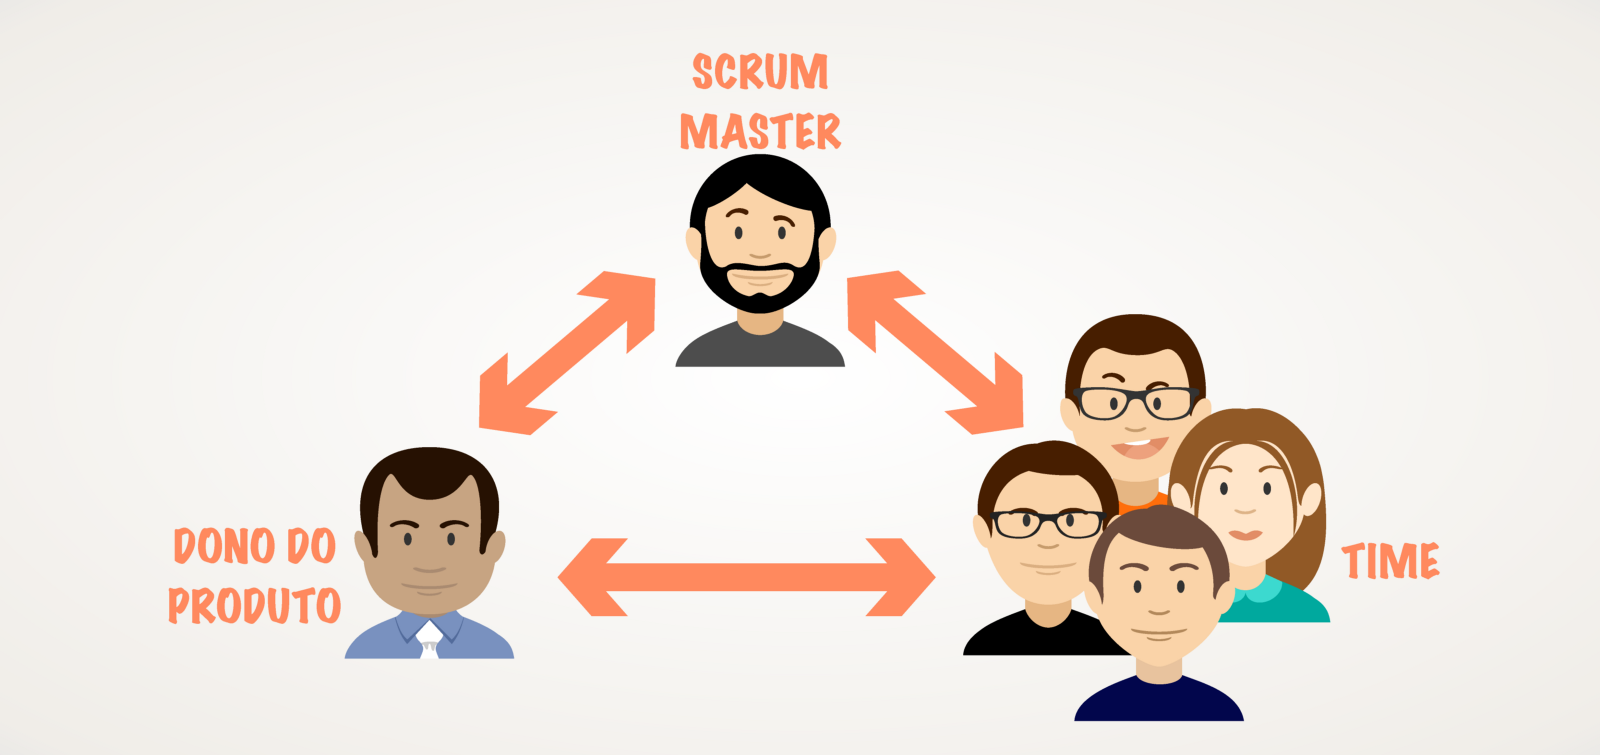
\includegraphics[width=1.0\textwidth]{figuras/papeis_scrum.png}
	\caption{Papéis Scrum. Fonte: \citeonline{papeis_scrum}.}
	\label{img:papeis_scrum}
\end{figure}

Como observado na figura \ref{img:papeis_scrum}, o \textit{Scrum} possui três papéis bem definidos: o \textit{Product Owner}, conhecido como PO, o \textit{Scrum Master} e por fim temos o \textit{Dev Team}. 

\subsubsubsection{Product Owner}

O \textit{Product Owner}, é o dono do produto. É ele que fornece o conhecimento do negócio em forma de requisitos para a equipe e na forma pratíca são os patrocionadores/clientes do produto. O PO organiza e prioriza o \textit{Product Backlog} (que são os itens que devem ser desenvolvidos), esse papel deve ser assumido por pessoas que sejam boas em se comunicar, pois esse papel é responsável por trabalhar e tirar dúvidas da \textit{Dev Team}.

\subsubsubsection{Scrum Master}

Ao analisar a figura \ref{img:papeis_scrum}, a figura do \textit{Scrum Master} parece ser superior aos outros papéis, o que não é verdade. O \textit{Scrum Master} possui o dever de ajudar a comunicação entre o PO e o \textit{Dev Team} além de remover todos os impedimentos que estão prejudicando o desenvolvimento, tem a função de auxiliar o amadurecimento da \textit{Dev Team} e promover as cerimônias que o \textit{Scrum} preza, como \textit{Daily Meetings}, \textit{Sprint Review} e \textit{Sprint Retrospective}.

\subsubsubsection{Dev Team}

Esse papel é voltada para as pessoas que de fato irão desenvolver o produto. O \textit{Dev Team} é auto-organizável e decide entre si como implementar os itens priorizados pelo PO.

\subsubsection{Scrum Solo}

Uma das adaptações do \textit{Scrum} é o \textit{Scrum} Solo, criado por \citeonline{scrum_solo} na UTFPR, Universidade Tecnológica Federal do Paraná. O \textit{Scrum} Solo é voltado para o desenvolvimento individual de \textit{software}, contudo sem seguir todos os rituais presentes no \textit{Scrum}, como visto no tópico \ref{sec:scrum}.

Ao final de uma \textit{Sprint}, um incremento de \textit{software} deve ser entregue assim como no \textit{Scrum}. Os artefatos de \textit{Product Backlog} e \textit{Sprint Backlog} são feitos da mesma maneira em ambos os casos. No \textit{Scrum} Solo como é desenvolvido individualmente, não há necessidade de reuniões diárias entre os membros como no \textit{Scrum}, havendo reunião somente quando necessário entre o desenvolvedor e o grupo de validação. Esse ciclo de vida pode ser visualizado na Figura \ref{img:ciclo_scrum_solo}:

\begin{figure}[H]
	\centering
	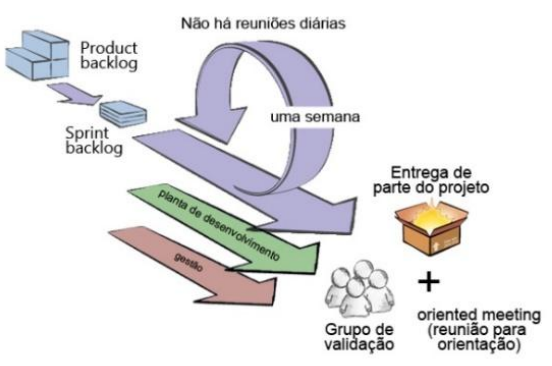
\includegraphics[width=0.9\textwidth]{figuras/fluxoScrumSolo.png}
	\caption{Ciclo de Vida \textit{Scrum} Solo. Fonte: \citeonline{scrum_solo}.}
	\label{img:ciclo_scrum_solo}
\end{figure}

As atividades do \textit{Scrum} Solo, segundo \citeonline{scrum_solo} são:

\begin{itemize}
	\item \textit{Requeriment}: definir escopo, caracterizar o cliente e definir o \textit{Product Backlog}; 
	\item \textit{Sprint}: selecionar o que será desenvolvido a partir do \textit{Sprint Backlog} em duração máxima de uma semana;
	\item \textit{Deployment}: tem como objetivo disponibilizar o produto para o cliente;
	\item \textit{Management}: planejar, monitorar e controlar o desenvolvimento do produto.
\end{itemize}

Segundo \citeonline{scrum_solo}, os atores envolvidos são:

\begin{itemize}
	\item \textit{Product Owner}: proprietário do produto;
	\item Desenvolvedor: responsável por executar o processo e desenvolver o produto;
	\item Orientador: consultor que conhece a fundo o processo;
	\item Grupo de validação: possíveis usuários do produto.
\end{itemize}

\section{Processo de Desenvolvimento de Software}
\label{sec:processo_de_desenvolvimento_de_software}

Segundo \citeonline{sommerville}, esse processo pode ser definido como "Um processo de \textit{software} é um conjunto de atividades relacionadas que levam à produção de um produto de \textit{software}."

Neste trabalho, foram definidas as principais atividades a serem realizadas para alcançar o objetivo final de ter um \textit{software} gratuito,código aberto e que auxilie os gerentes a otimizar suas reuniões por meio computacional são:

\begin{itemize}
    \item Especificação do \textit{software}: funcionalidades e restrições do \textit{software};
    \item Projeto e implementação do \textit{software}: as especificações que o \textit{software} deve atender;
    \item Validação de \textit{software}: para que atenda as expectativas do cliente, o \textit{software} deve ser validado pelo mesmo;
    \item Evolução do \textit{software}: o \textit{software} deve ser capaz de ser extensível a mudanças, tendo assim seu código aberto.
\end{itemize}

\subsection{Definição dos Requisitos}

Requisito não é um termo usado apenas pela \imprimircurso. Há casos em que requisitos são apenas uma declaração abstrata em alto nível de um serviço ou restrição que um sistema deve oferecer.

\citeonline{sommerville} os define como: "Os requisitos de um sistema são as descrições do que o sistema deve fazer, os serviços que oferece e as restrições a seu funcionamento. Esses requisitos refletem as necessidades dos clientes para um sistema que serve a uma finalidade determinada, como controlar um dispositivo, colocar um pedido ou encontrar informações."

\begin{figure}[H]
	\centering
	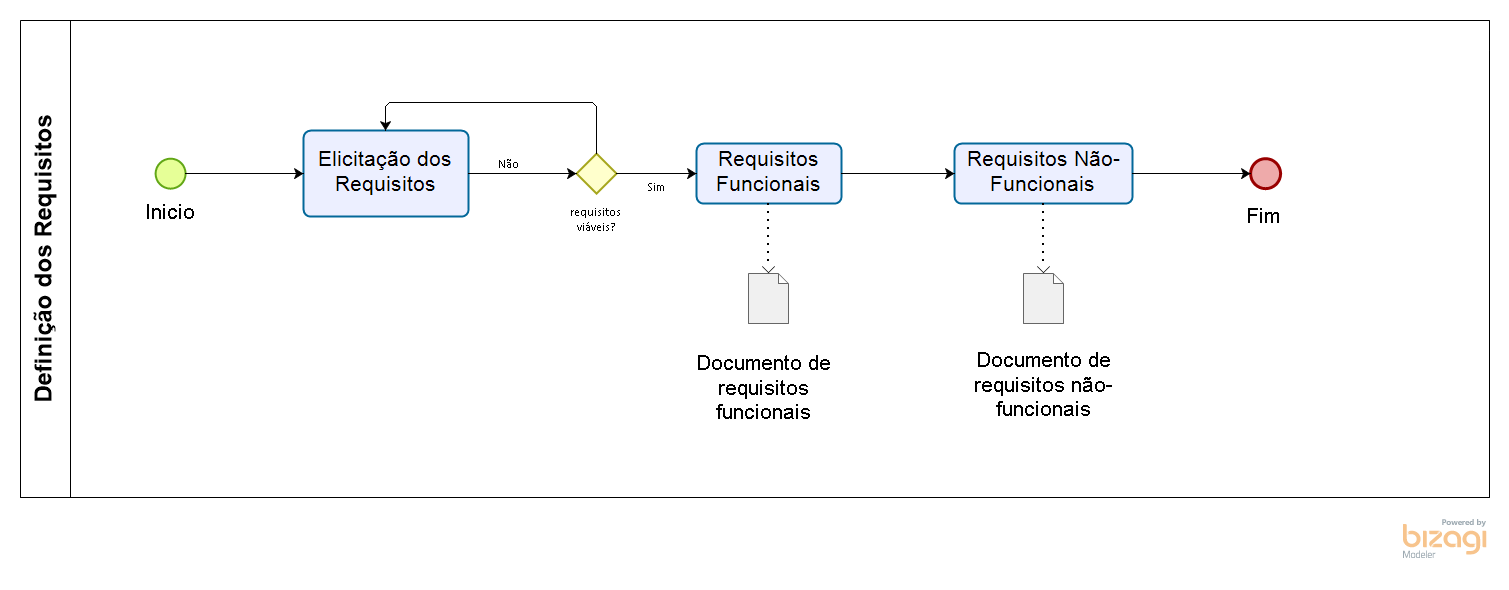
\includegraphics[width=1.0\textwidth]{figuras/elicitacaoDosRequisitos.png}
	\caption{Definição dos Requisitos. Fonte: Própria.}
	\label{img:definicao_requisitos}
\end{figure}

\subsubsection{Elicitação dos Requisitos}
\label{sec:elicitacao_requisitos}

\citeonline{sommerville} define a elicitação de requisitos como uma fase do projeto onde são extraídas informações do cliente sobre o que ele deseja que seja construído. É a fase em que o profissional de TI entende a necessidade do cliente e o orienta. É o momento de conversa com o usuário, de sentimento sobre o que este espera que seja entregue a ele. Na elicitação de requisitos são percebidas as necessidades do sistema e as características que esse sistema deve ter. Dentre todas as técnicas dentro da literatura, foram selecionadas duas como condidatas a serem usadas no projeto:

\begin{itemize}
    \item Entrevista
    \item Observação
\end{itemize}

\subsubsubsection{Entrevista}
\label{sec:entrevista}

Segundo \citeonline{sommerville}, as entrevistas podem ser formais ou não, mas fazem parte da maioria dos processos de engenharia de requisitos. Nas entrevistas, é realizada pela equipe de engenharia de requisitos perguntas aos \textit{stakeholders} sobre o sistema em vigor e o que será desenvolvido. A partir dessas perguntas surgem os requisitos.

As entrevistas podem ser de dois tipos: fechadas e abertas. Nas entrevistas fechadas, os \textit{stakeholders} respondem perguntas um conjunto de perguntas pré-definidas. Já nas entrevistas fechadas, são realizadas perguntas abertas sobre o sistema, e é nesse tipo de entrevista em que ocorre uma melhor compreensão das necessidades dos \textit{stakeholders}.  

\subsubsubsection{Observação}
\label{sec:observacao}

\cite{sommerville} define observação como uma técnica que pode ser usada para compreender os processos operacionais e ajudar a extrair os requisitos de apoio para esses processos. O trabalho do dia a dia é observado e são feitas anotações sobre as tarefas reais em que os partici­
pantes estão envolvidos. O valor da observação é que ela ajuda a descobrir requisitos implícitos do sistema que refletem as formas reais com que as pessoas trabalham, em vez de refletir processos formais definidos pela organização.

\subsubsection{Requisitos Funcionais}
\label{sec:requisitos_funcionais}

Os requisitos funcionais descreve o que o sistema deve de fato ser. Requisitos funcionais podem ser tão específicos quanto necessário,por exemplo, podem ter sistemas com requisitos funcionais gerais e outros que além de refletir os sistemas, também abrangem as formas de trabalho de uma organização. Requisitos funcionais de um sistema deve ser completo, isso quer dizer que todos os serviços requisitados pelo usuário devem ser definidos.

\subsubsection{Requisitos Não-Funcionais}
\label{sec:requisitos_nao_funcionais}

Requisitos não-funcionais são requisitos que são relacionados as propriedades do sistema como confiabilidade, tempo de espera, desempenho, segurança e até restrições do sistema. Requisitos não-funcionais podem possui tanta relevância quanto os requisitos funcionais, pois em uma reunião de levantamento de requisitos, o cliente sonha o mundo e não está atento se os recursos os próprios recursos e os recursos da emprega conseguem atender ao requisito. Um requisito não-funcional não atendido pode inclusive inutilizar um projeto. Exemplo disso é caso um sistema de uma aeronave não consiga atingir a confiabilidade necessária, não será dado o certificado de segurança para operar, sendo assim a aeronave não poderá voar.

\subsection{Linguagem de Software}

Linguagem de programação são instruções passadas de maneira que o computador entenda e apresente um retorno. Existem diversas linguagens de programação, desde a mais baixo a alto nível.

Linguagens de \textit{software}, como também podem ser chamadas, são divididas em duas frentes: \textit{front-end} e \textit{back-end}. Ambas serão explicadas nos tópicos a seguir.

\subsubsection{Front-end}
\label{sec:front-end}

A programação de um \textit{software} pelo ponto de vista do \textit{front-end} é a visão final do usuário com o sistema. \textit{Front-end} é a responsável pela interação do usuário com o sistema e essa interação é dada a partir de telas/páginas. Existem diversos tipos de \textit{frameworks} que auxiliam os desenvolvedores a trabalhar com essa frente, como:

\begin{itemize}
    \item \textit{Bootstrap
    \item Materialize
    \item ReactJs
    \item Angular 4}
\end{itemize}

\subsubsection{Back-end}
\label{sec:back-end}

A programação \textit{back-end} possui as responsabilidades de receber os dados pelo \textit{React}, que é o \textit{front-end} deste projeto, possui o dever de tratar os dados, valida-los e fomentá-los a visão do usuário.

Existem diversas linguagens \textit{back-end} que auxiliam os desenvolvedores a trabalhar em uma linguagem que o computador entende, como:

\begin{itemize}
    \item \textit{Python Django-Rest
    \item Java
    \item Ruby on Rails
    \item PHP}
\end{itemize}

Para este projeto foram escolhidas as linguagens de \textit{front-end} o \textit{ReactJs} e para \textit{back-end} o \textit{Python Django-Rest}.

\subsubsection{Arquitetura de Software}

A arquitetura de \textit{software} é como o sistema deve ser organizado com a estrutura geral do projeto. A arquitetura possui um valor alto dentro da construção de um \textit{software}, pois nela se tem o elo entre o projeto e a engenharia de requisitos. Possui o dever identificar os principais componentes estruturais no sistema e o relacionamento entre eles.

\subsubsection{Model-View-Controller}
\label{sec:mvc}

O padrão arquitetural MVC é responsável de responsabilidades em camadas. A primeira é \textit{Model}(modelo), que é responsável pela manipulação de dados, ou seja, leitura, escrita de dados e também suas validações é de responsabilidade da Model. A segunda camada é a \textit{View}(visão), que possui a responsabilidade de interação com o usuário. Por último se tem a \textit{Controller}(controladora), responsável por receber as aquisições do usuário. A controller também tem o dever de disponibilizar os dados para a \textit{view} e assim ocorrer a interação com o usuário.